% Document class
\documentclass{article}

% For figures
\usepackage{graphicx} % more modern
\usepackage{subfigure} 

% For citations
\usepackage{natbib}

% For algorithms
\usepackage{algorithm}

% algorithmic like to break pdflatex(probably ancient package), use at own risk
% \usepackage{algorithmic}

% As of 2011, we use the hyperref package to produce hyperlinks in the
% resulting PDF.  If this breaks your system, please commend out the
% following usepackage line and replace \usepackage{cs4437cs9637} with
% \usepackage[nohyperref]{cs4437cs9637}
\usepackage{hyperref}

% Packages hyperref and algorithmic misbehave sometimes.  We can fix
% this with the following command.
\newcommand{\theHalgorithm}{\arabic{algorithm}}

\usepackage{cs4437cs9637} 

\begin{document}

% The \cstitle you define below is probably too long as a header.
% Therefore, a short form for the running title is supplied here:
\cstitlerunning{Report Draft}

\twocolumn[
\cstitle{Evaluating Solution Quality and Problem Difficulty Utilizing Code
Metrics}

% Author information
\csauthor{Gurpreet Singh (\normalsize\emph{\# 250674134})}{\href{mailto:gsingh95@uwo.ca}{\nolinkurl{gsingh95@uwo.ca}}}
\csaddress{The University Of Western Ontario}

% You may provide any keywords that you 
% find helpful for describing your paper; these are used to populate 
% the "keywords" metadata in the PDF but will not be shown in the document
\cskeywords{}

\vskip 0.3in
]

\begin{abstract} 
{\bf Discovering the effects of code style on code functionality and problem
structure.} This study aims to showcase how well formatted, reusable and
maintainable code is fundamentally better in all circumstances by
looking at over 1 million results from a competitive programming website
and analyzing the correlation between question and solution. The goal is
to promote code quality checking in online `just in time' teaching
resources to improve the performance of interviewers, researchers, and
students. \end{abstract} 


\section{Description of Applied
Problem}\label{description-of-applied-problem}

\subsection{Problem identification}\label{problem-identification}

A large amount of educational material related to programming exists on
the internet but the majority of which is not well structured or
presented. An applied problem that can be observed from educational
material found online is that code quality is often left mutually
exclusive from code functionality. \citet{justintimeteaching}

This leads to some students believing it is acceptable to write code
that produces the correct result even if the process behind it is not
correct. Online code challenge websites like CodeChef.com do not take
into account the style and quality metrics of a code submission when
judging competitions. \citet{codechef} Cutting corners in the learning
process advances into a complete disregard for best practices in open
source software and in the workplace which results in a larger amount of
errors. Readability of code is an essential metric in software
engineering and can be improved even with simple additions of whitespace
between lines. \citet{codereadability}

Computer code written by researchers and other individuals who are just
trying to accomplish a result in any way possible is often of the worse
quality. This is because they learn using the `just in time' mentality
and the resources online that promote this mentality disregard code
quality. \citet{justintimeteaching} Lack of code quality directly
reduces it's re-usability because other programmers have a harder time
understanding what the code is doing. If these teaching resources could
use questions and checks that promote better code quality, many
technical innovations could be made. Researchers would be more educated
on how to create reusable code and this would influence developers to
take their ideas and apply them to real life use cases.
\citet{reusability}

Code quality post processing software is often used in production
development environments to ensure good style choices. These checks are
much less useful at this senior level than they would be at an
educational level. If programming style can be judged on a submission,
companies conducting technical interviews will be able to better judge
applicants and make a more informed decision.

This study will focus on proving that code quality can have an influence
on code functionality, as well as which kinds of questions influence
good or bad code styles.

\subsection{Approach Strategy}\label{approach-strategy}

A solution to these problems is linking the scoring process in
programming problems to a metric derived from running code quality
checks on the submission.

Not only will this analysis benefit educational institutes but also
companies and competitions that judge people on their code submissions.

\section{Data Description}\label{data-description}

\subsection{CodeChef Dataset}\label{codechef-dataset}

CodeChef.com is a competitive programming web application that has
posted all of their questions and solutions onto the data science
website, Kaggle. The data consists of a questions comma separated file,
a solutions comma separated file and 3 files that show the code
associated with each solution id. The set contains about 1000 problem
statements and over 1 million code solutions submitted. This should be a
more than sufficient to make a training and test data set.

\subsection{Code Submission Language
Density}\label{code-submission-language-density}

The code submissions are written in many different programming languages
and each language has it's own code analysis tool. Therefore, to make
the process simpler and come up with higher quality results, the data
will need to be filtered by the top languages used.
Figure\textasciitilde{}\ref{languages} shows that C++, Java, C and
Python are the most popular submissions in this dataset. The majority of
the dataset is describing submissions in the C family of languages. They
are also the easiest to group together and process allowing for fair
comparison of results, therefore, this study will focus only on the C
family.

\begin{figure}[ht] \vskip 0.2in \begin{center}
\centerline{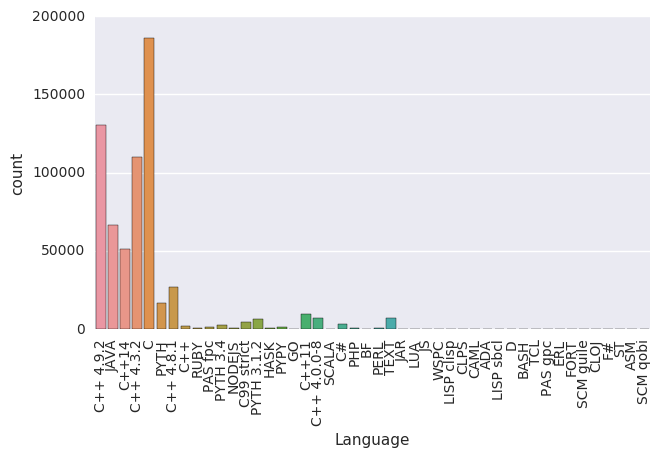
\includegraphics[width=\columnwidth]{../images/languages.png}}
\caption{Frequency of each programming language that occurs in the dataset of
solutions } \label{languages} \end{center} \vskip -0.2in \end{figure}

\citet{kernalnlp}

\subsection{Feature Selection}\label{feature-selection}

\subsubsection{Question Data}\label{question-data}

The most useful features in the question data files are title, link,
difficulty level, question statement, and time limit

\subsubsection{Solution Data}\label{solution-data}

The most useful features in the solution data files are status, time
taken, memory taken, and language

\subsubsection{Code Data}\label{code-data}

The code data files only contain two columns, the first one containing
the solution ID and the second containing the code string. The solution
ID will be used to merge the data with the solution data file and that
data frame will act as the base for the rest of the analysis on code.

In order to make the connection between code functionality and code
style, a large part of the experiment is obtaining an accurate and
unbiased metric for code quality. The decision to narrow the dataset to
only the C family shows it's importance here as we can use a single tool
to evaluate quality

The tool we will be using is \texttt{cpplint}. It is open source and
follows
\href{https://google.github.io/styleguide/cppguide.html}{Google's C
style guide}

\subsection{Code Equivalence}\label{code-equivalence}

\section{Visualizations}\label{visualizations}

\bibliography{bibliography.bib}
\bibliographystyle{plainnat}

\end{document} 
